%---------------------------------------------------------------------------%
%-                                                                         -%
%-                           LaTeX Template                                -%
%-                                                                         -%
%---------------------------------------------------------------------------%
%- Copyright (C) Huangrui Mo <huangrui.mo@gmail.com> 
%- This is free software: you can redistribute it and/or modify it
%- under the terms of the GNU General Public License as published by
%- the Free Software Foundation, either version 3 of the License, or
%- (at your option) any later version.
%---------------------------------------------------------------------------%
%->> Document class declaration
%---------------------------------------------------------------------------%
\documentclass[doublesided]{Style/ucasthesis}%
%- Multiple optional arguments:
%- [<singlesided|doublesided|printcopy>]% set one or two sided eprint or print
%- [draftversion]% show draft version information
%- [fontset=<fandol|...>]% specify font set to replace automatic detection
%- [scheme=plain]% thesis writing of international students
%- [standard options for ctex book class: draft|paper size|font size|...]%
%---------------------------------------------------------------------------%
%->> Document settings
%---------------------------------------------------------------------------%
\usepackage[super,myhdr,list]{Style/artratex}% document settings
%- usage: \usepackage[option1,option2,...,optionN]{artratex}
%- Multiple optional arguments:
%- [bibtex|biber]% set bibliography processor and package
%- [<numbers|super|authoryear|alpha>]% set citation and reference style
%- <numbers>: textual: Jones [1]; parenthetical: [1]
%- <super>: textual: Jones superscript [1]; parenthetical: superscript [1]
%- <authoryear>: textual: Jones (1995); parenthetical: (Jones, 1995)
%- <alpha>: textual: not available; parenthetical: [Jon95]
%- [geometry]% reconfigure page layout via geometry package
%- [lscape]% provide landscape layout environment
%- [myhdr]% enable header and footer via fancyhdr package
%- [color]% provide color support via xcolor package
%- [background]% enable page background
%- [tikz]% provide complex diagrams via tikz package
%- [table]% provide complex tables via ctable package
%- [list]% provide enhanced list environments for algorithm and coding
%- [math]% enable some extra math packages
\usepackage{Style/artracom}% user defined commands

\let\openbox\relax
\usepackage{amsthm}
%-------------我的-----------------------------------------------------------%
\usepackage{proof}
\usepackage{listings}
\usepackage{color}
%---------------------------------------------------------------------------%
%->> 对于数学定理的表示
\theoremstyle{plain}
\newtheorem{thm}{定理}[section]
\newtheorem{lem}[thm]{引理}
\newtheorem{prop}[thm]{命题}
\newtheorem{cor}{推论}

\theoremstyle{definition}
\newtheorem{defn}{定义}[section]
\newtheorem{conj}{猜想}[section]
\newtheorem{exmp}{示例}[section]

\theoremstyle{remark}
\newtheorem*{rem}{标注}
\newtheorem*{note}{注解}

\newenvironment{pf}{{\noindent\it 证明.}\quad}{\hfill $\square$\par}
%---------------------------------------------------------------------------%
%->> Document inclusio
%---------------------------------------------------------------------------%
%\includeonly{Tex/Chap_1,...,Tex/Chap_N}% selected files compilation
%---------------------------------------------------------------------------%
%->> Document content
%---------------------------------------------------------------------------%
\begin{document}
	%-
	%-> Frontmatter: title page, abstract, content list, symbol list, preface
	%-
	\frontmatter% initialize the environment
	%---------------------------------------------------------------------------%
%->> 封面信息及生成
%---------------------------------------------------------------------------%
%-
%-> 中文封面信息
%-
%\confidential{}% 密级:只有涉密论文才填写

%-


%-
%-> 作者声明
%-
%\makedeclaration% 生成声明页
%-
%-> 中文摘要
%-

\chapter*{摘\quad 要}\chaptermark{摘\quad 要}% 摘要标题
\setcounter{page}{1}% 开始页码
\pagenumbering{Roman}% 页码符号
多方安全计算(Secure Multi-party Computation,简称为SMPC)是安全计算的一个前沿研究领域。它研究如何使互不信任的多个参与者,在不泄露自身隐私输入数据信息的前提下,协同计算一个依赖各个参与者输入数据的函数的结果。Wys*是第一个用于开发SMPC程序的领域特定语言。Wys*基于F*面向验证的特点,拥有对Wys*开发的SMPC程序进行计算正确性和安全性验证的能力,并完成了自身的形式化验证。本文以完善对多方安全计算程序的验证能力为出发点,对Wys*的结构进行分析发现Wys*将多方安全计算函数编译为布尔电路时没有进行检查,导致可能在电路编译时出现错误。根据此观察提出基于类型的验证方法Wys-ckt,Wys-ckt对Wys*程序中的多方安全计算函数进行验证,保证安全计算函数的语义符合Wys*的电路编译能力。  


\keywords{多方安全计算,程序验证,电路编译,类型系统}% 中文关键词
%-
%-> 英文摘要
%-
\chapter*{Abstract}\chaptermark{Abstract}% 摘要标题

Secure multi-party computation(SMPC) is a research area of secure computation. SMPC makes participators learn the correct output of a public function on their private data while keeping their own inputs secret. Wys* is the first domain specific language used for SMPC programs. Wys* is based on the verification-oriented property of F* language. It is able to verify the computation correctness and security reliability of SMPC programs and it is also formally verified itself. This thesis is aimed to improve the verification ability to SMPC programs. While analyzing the structure of Wys*, one of what we find is that Wys* doesn't check the public secure function when compile this function to boolean circuit so that an error may occur during the circuit compiling process. Based on this observation, we design and implement a type-based verification tool called Wys-ckt. Wys* has an ability to verify the public secure function of a Wys* progam so that ensure the semantic of the public secure function is under the circuit compiling ability of Wys*. 

\englishkeywords{secure multi-party computation, program verification, circuit translation, type system}% 英文关键词
%---------------------------------------------------------------------------%
% title page, abstract, dedication
	{% content list region
		\linespread{1.2}% local line space
		%\intotoc{\contentsname}% add link to contents table and bookmark
		\tableofcontents% contents catalog
		%\intotoc{\listfigurename}% add link to contents table and bookmark
		%\listoffigures% figures catalog
		%\intotoc{\listtablename}% add link to contents table and bookmark
		%\listoftables% tables catalog
	}
	%\chapter*{符号列表}
\chaptermark{符号列表}

\section*{字符}
\nomenclatureitem[\textbf{Unit}]{\textbf{Symbol}}{\textbf{Description}}
\nomenclatureitem[$\Unit{m^{2} \cdot s^{-2} \cdot K^{-1}}$]{$R$}{the gas constant}
\nomenclatureitem[$\Unit{m^{2} \cdot s^{-2} \cdot K^{-1}}$]{$C_v$}{specific heat capacity at constant volume}
\nomenclatureitem[$\Unit{m^{2} \cdot s^{-2} \cdot K^{-1}}$]{$C_p$}{specific heat capacity at constant pressure}
\nomenclatureitem[$\Unit{m^{2} \cdot s^{-2}}$]{$E$}{specific total energy}
\nomenclatureitem[$\Unit{m^{2} \cdot s^{-2}}$]{$e$}{specific internal energy}
\nomenclatureitem[$\Unit{m^{2} \cdot s^{-2}}$]{$h_T$}{specific total enthalpy}
\nomenclatureitem[$\Unit{m^{2} \cdot s^{-2}}$]{$h$}{specific enthalpy}
\nomenclatureitem[$\Unit{kg \cdot m \cdot s^{-3} \cdot K^{-1}}$]{$k$}{thermal conductivity}
\nomenclatureitem[$\Unit{kg \cdot m^{-1} \cdot s^{-2}}$]{$S_{ij}$}{deviatoric stress tensor}
\nomenclatureitem[$\Unit{kg \cdot m^{-1} \cdot s^{-2}}$]{$\tau_{ij}$}{viscous stress tensor}
\nomenclatureitem[$\Unit{1}$]{$\delta_{ij}$}{Kronecker tensor}
\nomenclatureitem[$\Unit{1}$]{$I_{ij}$}{identity tensor}

\section*{算子}
\nomenclatureitem{\textbf{Symbol}}{\textbf{Description}}
\nomenclatureitem{$\Delta$}{difference}
\nomenclatureitem{$\nabla$}{gradient operator}
\nomenclatureitem{$\delta^{\pm}$}{upwind-biased interpolation scheme}

\section*{缩写}
\nomenclatureitem{CFD}{Computational Fluid Dynamics}
\nomenclatureitem{CFL}{Courant-Friedrichs-Lewy}
\nomenclatureitem{EOS}{Equation of State}
\nomenclatureitem{JWL}{Jones-Wilkins-Lee}
\nomenclatureitem{WENO}{Weighted Essentially Non-oscillatory}
\nomenclatureitem{ZND}{Zel'dovich-von Neumann-Doering}

% list of symbols, preface content
	%-
	%-> Mainmatter
	%-
	\mainmatter% initialize the environment
	%---------------------------------------------------------------------------%
%->> Main content
%---------------------------------------------------------------------------%
\chapter{绪论}\label{chap:introduction}
本章介绍本文的研究背景、目的和结果。第一节概括性的介绍多方安全计算问题、协议、程序和验证。第二节举例介绍了多方安全计算程序验证方面的研究情况,并提出本文研究的Wys*程序安全计算函数的编译可行性问题。第三节详细说明了本文研究的具体问题以及基于类型检查的研究方法和对示例程序的测试结果。
\section{背景介绍}
随着互联网技术的普及应用,不同的应用场景都在寻找合适的互联网解决方案。其中一类需要由可信第三方作为中间担保人来保护参与者隐私的诸多实际传统应用和新型网络应用,例如无记名投票、碱基序列比较、数据库的私有查询、隐私集合求交集等,利用多方安全计算技术得以实现在免除第三方中间人的需要的同时满足高隐私保护性,避免由于第三方担保人的失误导致的安全问题和对第三方可信赖程度的担忧。

多方安全计算最早在1982年由姚智期在百万富翁问题中提出。百万富翁问题是两方安全计算问题的一个简单实例,表述为如何在不借助第三个人的情况下,使两个百万富翁比较出谁更富有并且彼此不让对方得知自己的财富数量。姚智期随后提出了解决任意两方安全计算的混淆电路协议(Garbled Circuits Protocol)方法\citep{yao1982protocols}。Goldreich等人将两方计算问题进行拓展,与1987年系统性的阐述了多方安全计算问题,并提出了基于秘密共享(Secret Sharing)的GMW协议\citep{goldreich2019play}(Goldreich-Micali-Wigderson Protocol)。多方安全计算解决的问题是如何使互不信任的参与者,在保证各自隐私数据不被泄漏的情况下,协同计算一个结果依赖于各方隐私数据的函数。SMPC协议发展至今出现了许多高效可靠的技术用于提高SMPC的计算效率,也出现了结合混淆电路和秘密共享两种方案长处的混合协议,专用于开发多方安全计算程序的框架也被开发出来,SMPC得以逐渐在实际问题中应用。

在软件安全领域,对多方安全计算程序的形式化验证也受到了研究者的关注,近年来出现了基于语言的SMPC程序验证方案SecreC\citep{almeida2018enforcing}和Wys*\citep{rastogi2019textsc}。这两种方案从不同的角度对SMPC程序的部分性质进行了验证,虽然各自都有一些缺点,但是为语言层面的SMPC程序验证工作打开了思路。本文以Rastogi等人提出的SMPC程序的领域特定语言Wys*\citep{rastogi2019textsc}为研究对象,Wys*最大的特点是面向程序验证,相比于SecreC\citep{almeida2018enforcing}等其他SMPC验证工作,Wys*依托于F*的逻辑推理和证明能力,能够对程序的计算正确性和安全性进行验证。Wys*是首个SMPC程序的领域特定语言(Domain Specific Language),基于对Wys*的分析发现存在一些有待改进的缺点,其中的一个缺点就是Wys*没有对从代码到电路的编译时可行性进行检查,导致经过验证的Wys*程序在实际运行时可能因为电路编译失败出现运行时错误,这个缺点在SecreC中也同样存在。基于此观察,本文设计开发对Wys*程序中的安全计算函数进行电路编译的可行性进行检查的方法,作为Wys*和SMPC验证的有益补充。
\section{SMPC验证的发展现状}\label{sec:system}
Backes等人\citep{backes2010computationally}早在2010年利用Applied $\pi$-calculus方法对SMPC协议模型进行符号抽象,并基于类型检查的方法提出一种对符号抽象后的SMPC协议模型的正确性进行形式化验证的方法。此方法验证SMPC在协议层面的可靠性,但进行了切实可行的设计实现和实验。 随后Almeida等人\citep{almeida2018enforcing}提出了基于语言的验证SMPC程序隐私数据安全性的验证方法,在Sharemind\citep{bogdanov2008sharemind}安全计算框架中的SecreC(类似C++ 的商业性SMPC语言)基础上,加入特殊的解密操作符declassify,并将数据和运算符都分为public和private类型,然后建立了隐私数据泄漏情况推理系统。SecreC允许设定数据泄漏的阈值函数,在分析SecreC的程序信息流(Information Flow)过程中用于进行检查,验证SecreC编写的SMPC程序对隐私数据的保护程度是否满足所设定的隐私泄漏阈值。Rastogi等人\citep{rastogi2019textsc}提出的Wys*是一种SMPC领域特定语言,Wys*基于F*(由微软研究院和法国国家信息与自动化研究所主导开发的面向验证的函数式语言),继承了F*的逻辑推理功能(Logic Inference),精化类型系统(Refinement Type System)和条件预言(Predicate)等为程序验证服务的功能。Wys*的设计使其能够对SMPC程序的计算正确性、安全性进行证明,同时也兼顾加入了用于开发高性能SMPC程序的特殊功能。

上述提到的主要是基于语言层面进行SMPC验证的工作,这些工作的目的都是验证SMPC程序的安全性质,但是显然不可能包含SMPC程序的所有安全性质,研究的具体内容各有偏向:Backes等人的研究关注SMPC协议模型在协议层面的正确性;Almeida等人的研究关注于SMPC程序在计算时的隐私保护能力,寻求在减少SMPC程序的协议交互,提高SMPC程序性能的同时依然保持合理的数据隐私保护能力;Rastogi等人的研究更关注于Wys*本身的形式化验证,从语言基础的层面保证SMPC程序的计算正确性和安全性。但是各个方案也都有明显的不足之处,以本文研究的Wys*为例,Wys*中使用的电路编译模块和GMW协议模块都不在Rastogi等人的工作的验证范围之内,其他地方也仍有不足,在实际应用中都是不安全的因素。

\section{本文的目的、方法及主要结果}
Rastogi等人的工作开发的Wys*具备进行完整、高效验证SMPC程序的能力,但是本身明显也能看到不足之处。通过对Wys*的设计内容和结构实现的详细分析,我们发现Wys*程序在运行时需要将程序中的安全计算函数编译为布尔电路,但是Wys*没有对这一部分函数进行检查,导致存在程序运行时电路编译失败而出现程序错误的可能,本文因此提出Wys-ckt工具。Wys*程序中的安全计算函数需要被编译为电路,Wys-ckt对这部分函数进行验证,验证这部分函数的语义没有超出Wys*的电路编译能力。Wys-ckt工具保证了经过Wys-ckt验证的程序中的安全计算函数一定能被Wys*顺利的编译为电路,避免了Wys*程序在运行时由于安全计算函数的语义超出的电路编译能力而出现的程序异常。

本文工作在推进时遇到一些难以解决的困难,一方面F*目前仍处于快速迭代中,尚没有公开完整的语法和类型系统,只能从教程和源码中获取主要语法;另一方面,Wys*依赖于特定的F*版本,所依赖的F*版本为非正式版,存在尚未修复的问题。因此,本文将Wys*看作F*的派生语言,根据Rastogi等人发表的与Wys*相关的文献\citep{rastogi2017wys, rastogi2014wysteria,rastogi2019textsc}中公开的特殊语法及类型,设计和实现了Wys*语言的程序文法分析器、静态类型分析以及电路编译可行性验证系统。

简单的Wys*程序经过F*验证系统的验证之后,几乎不需要修改就能在Wys-ckt中进行电路翻译条件满足性的验证。较为复杂的Wys*程序,由于F*语言设计中计算部分与验证部分保持分离的特点,经过F*的验证之后,将计算部分输入Wys-ckt中也能完成验证。

本文以Wys*中的三个SMPC程序示例:mill,median,psi为例进行实验。mill是一个百万富翁问题的程序实例;median是一个两方各输入两个整数求中位数的程序实例;psi是一个集合求交集问题的程序实例。我们在一台主频为2.30GHz的i5-6300HQ处理器平台上运行的Ubuntu 18.04系统当中对这三个程序示例的进行测试。测试结果如表\ref{tab:result}所示, 表中行数一栏代表不同程序源代码的行数,时间一栏代表Wys-ckt对一个程序进行三次分析验证需要花费时间的平均值,最大占用内存代表验证一个程序期间Wys-ckt占用内存的最大值,结果一栏表示Wys-ckt对程序的类型分析结果和验证结果是否符合预期。
\begin{table}[!htbp]
    \caption{Wys-ckt测试结果}
    \label{tab:result}
    \centering
    \footnotesize% fontsize
    \setlength{\tabcolsep}{4pt}% column separation
    \renewcommand{\arraystretch}{1.2}%row space 
    \begin{tabular}{lccccc}
        \hline
        程序示例 & 行数 & 时间(秒) & 最大占用内存(MB) & 结果 \\
        %\cline{2-9}% partial hline from column i to column j
        \hline
        mill   & $21$ & $0.005$ & $2.97$ & 正确 \\
        median & $51$ & $0.007$ & $3.11$ & 正确 \\
        psi    & $46$ & $0.007$ & $2.95$ & 正确 \\
        \hline
    \end{tabular}
\end{table}

根据\ref{tab:result}中的结果,Wys-ckt的实际表现符合设计预期。Wys-ckt的运行时间包含对整个输入程序的分析和对安全计算函数的验证两部分。因此随着输入程序规模的增长,Wys-ckt的运行时间随之增加。Wys-ckt占用的内存主要来自类型分析时存储的数据信息,随着输入程序中表达式数量的增加,Wys-ckt占用的内存呈现近似线性的增长。
\begin{figure}[!htbp]
    \centering
    \begin{subfigure}[b]{0.4\textwidth}
      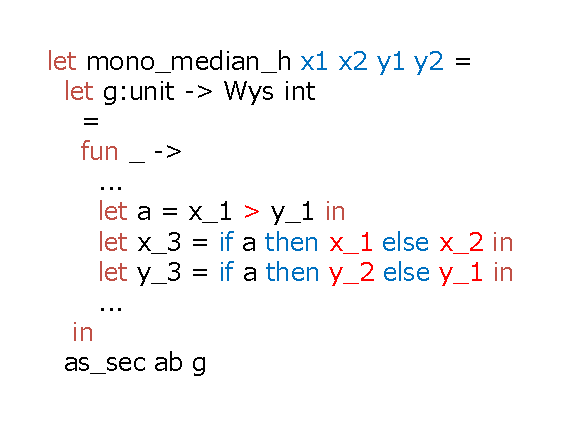
\includegraphics[width=\textwidth]{code.pdf}
      \caption{}
      \label{fig:code}
    \end{subfigure}%
    ~%add desired spacing
    \begin{subfigure}[b]{0.4\textwidth}
      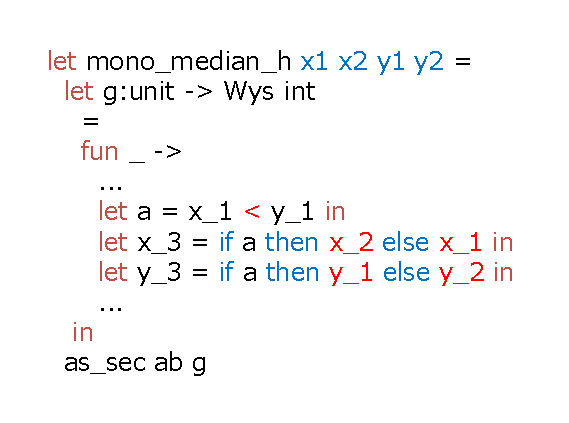
\includegraphics[width=\textwidth]{code2.pdf}
      \caption{}
      \label{fig:code2}
    \end{subfigure}
    \caption{(a) median原始代码的一部分,(b) 经过修改的median代码.}
    \label{fig:codeall}
\end{figure}

表\ref{tab:result}中三个例子都是Wys*提供的能够经过验证编译的程序,Wys-ckt的测试结果也正确的分析出了程序中语法树、类型与验证结果。接下来展示一个有电路编译错误的例子,图\ref{fig:code}中的内容是一段median例子中安全计算函数的一部分代码,将这段代码稍微修改得到图\ref{fig:code2}中的代码,两段代码的6-8行的内容不完全相同,但是却有完全等价的逻辑功能。将median中的图\ref{fig:code}展示的这部分代码修改为图\ref{fig:code2}中的内容后,新的median程序依然能够通过F*的验证,但是在运行时却会因为第6行的布尔比较操作符(<)不在Wys*的电路接受的操作符之内,会产生程序错误。类似这样的错误在一个不熟悉Wys*内部实现细节的多方安全计算程序开发人员的开发过程中是十分容易出现的。但是新的median经过Wys-ckt验证时,Wys-ckt可以发现这个问题并给出警告。通过以上对两种不同类型的例子的实验,证明了Wys-ckt工具的程序实现达到了Wys-ckt设计的预期功能,拥有验证Wys*程序中安全计算函数电路编译可行性的能力,Wys-ckt设计的验证条件保证了一个经过Wys-ckt验证的程序中的安全计算函数一定没有超过Wys*的电路编译能力。
\section{论文的结构}
本文的第二章是预备知识,详细介绍多方安全计算程序的执行过程,领域特定语言Wys*的特性和Wys*进行电路翻译的方法。

第三章重点介绍Wys-ckt的整个设计方案。第三章中将Wys*与F*进行合并,构建了本文研究的Wys*较为形式的语法系统,并且根据类型系统设计的原则将Wys*的特性加入进经典的类型系统当中,最后基于类型设计了电路翻译条件的验证系统,从理论上完成了Wys-ckt的构建。

第四章介绍本文如何将Wys-ckt的理论系统进行实现。Wys-ckt的实现基于O-caml,与F*同属ML家族,利用模式匹配特性可以方便的构建分析作用的代码。本文实现的大部分篇幅用于构建一个完善的拥有类型系统的语法树,然后按照第三章设计的验证模式进行验证。 

\chapter{预备知识}\label{Guide}
本章详细说明本文研究所需要掌握的基础知识。第一节解释了多方安全计算问题的定义和需要满足的性质以及多方安全计算程序的执行过程。第二节较为完整的说明了Wys*的特性,实现安全计算的方法以及特殊结构的功能。第三节介绍了Wys*的电路编译过程并给出了Wys*语法中能够进行电路编译的语法子集。
\section{多方安全计算}
在一个SMPC定义中\citep{evans2017pragmatic},一组$n$个参与者$p_1,p_2,\dots,p_n$各自拥有隐私数据$d_1,$ $d_2,\dots,d_n$。参与者们在计算一个依赖于各方隐私数据的公开函数$f(d_1,d_2,\dots,d_n)$ 的同时保持各自输入的$d_i$的隐秘性。基于完全可信的第三方的解决方案十分朴素,由第三方$s$分别接受各个参与者的输入$d_i$,由$s$计算出$f(d_1,d_2,\dots,d_n)$的结果$z$后,返回$z$给各个参与者$p_i$。完全可信的第三方是不存在的,因此基于可信第三方的解决方案带来的问题是显而易见的。使用技术手段解决SMPC问题的途径有两种,一种是基于可信硬件(例如Intel SGX),另一种是基于密码学协议的多方安全计算协议(例如GMW协议,BMR协议等),本文介绍基于多方安全计算协议的多方安全计算。基于完全可信的第三方是最理想情况下的解决方案,在该方案下的计算过程中,每个参与者$p_i$得到的信息只有各自的输入$d_i$以及计算结果$z$,此外没有任何的额外信息能够用于推测其他参与者的输入。多方安全计算协议为了达到安全性至少需要满足两个属性:
\begin{itemize}
	\item 输入数据$d_i$的隐私性。计算过程中$p_i$获得的除$d_i$和$z$以外的任何中间数据对于推测其他参与者的输入没有任何帮助。
	\item 正确性。任何参与者的作弊行为或联合作弊行为都不能迫使诚实的参与方获得错误的结果$z$,这意味着计算结束时诚实的参与者一定能得到正确的结果,否则协议会在计算结束前中止。
\end{itemize}

多方安全计算协议发展至今,姚智期的混淆电路协议、GMW协议\citep{goldreich2019play}、BMR协议\citep{beaver1990round}等诸多协议在不同的安全假设下实现了多方安全计算,此外还出现了为特定的多方安全计算问题专门优化的协议,如解决隐私集合求交集问题的PSSZ协议\citep{pinkas2015phasing}等。我们将基于多方安全计算协议开发的用于解决多方安全问题的程序称为多方安全计算程序,目前已有许多用于开发多方安全计算程序的框架,如Sharemind、Wysteria、Obliv-C等\citep{bogdanov2008sharemind, rastogi2014wysteria, zahur2015obliv},这些框架整合了多方安全计算程序需要的网络和密码学程序库、多方安全计算协议实现、电路编译器、程序解释器等组件,提供了不同需求场景下的多方安全计算程序开发平台。

一个多方安全计算程序的执行包含许多过程,如图\ref{fig:smpc}。一般来说,当解释器解释执行一个多方安全计算程序时,本地计算内容在本地完成,多方计算函数先被编译为布尔电路或算术电路,然后作为多方安全计算协议的输入,主程序此时暂停执行,等待获得多方计算的结果后再继续执行。多方协议执行时通过网络与各方进行通信,等待各方协议执行完成进行同步再将结果返回给主程序。
\begin{figure}[!htbp]
    \centering
    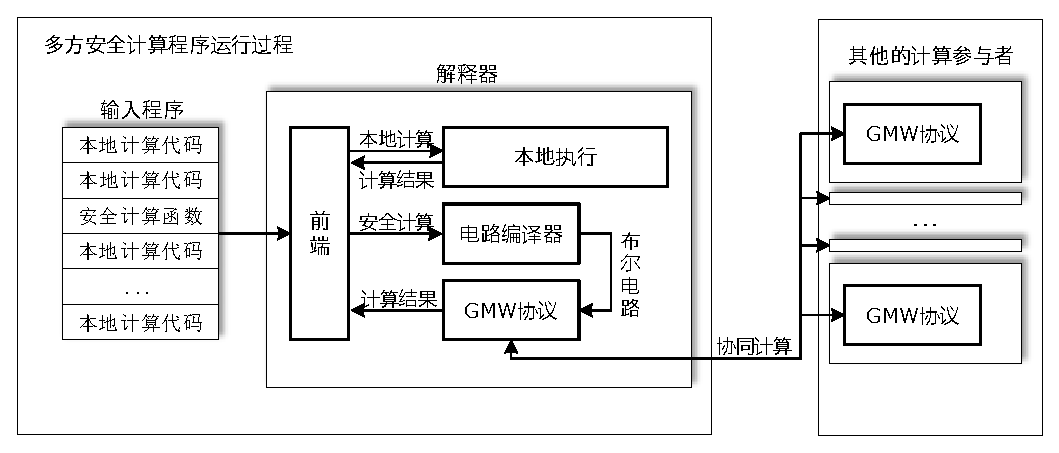
\includegraphics[width=1.00\textwidth]{SMPC.pdf}
    \caption{多方安全计算程序的执行过程}
    \label{fig:smpc}
\end{figure}

\section{Wys*:多方安全计算领域特定语言}
Wys*是Aseem Rastogi等人设计和开发的面向验证的多方安全计算的领域特定语言,Wys*的前身是同样用于开发多方安全计算程序的Wysteria\citep{rastogi2014wysteria}。Wys*底层使用拥有丰富验证功能的Fstar,在完成了前身Wysteria的功能同时完成了对自身的形式化验证。Wys*中利用联合类型声明了一类用于区分不同参与者标识的关键字Alice,Bob,Charlie等,这些标识除了区别参与者身份外,还被用于区别不同参与者来源的数据以及限制隐私数据的访问权限。 

Wys*有两个最重要的特点\citep{rastogi2019textsc}:
\begin{itemize}
	\item Wys*为SMPC设计了清晰的程序逻辑:Wys*的程序设计为混合模式,由本地计算,程序交互和安全计算三种模式组成。Wys*的程序模式使应用程序可以编写为与分布式语义等价的单线程语义的形式,解决了不同参与方各自拥有一份不同实现的情况。基于Fstar的验证能力,Wys*在程序中嵌入前置条件和后置条件来检查程序逻辑,并为检查用户指定的安全属性提供了可供观察的信息。
	\item Wys*实现了丰富的功能,其中一部分经过形式化验证。Wys*使用解释器在本地执行本地计算,安全计算函数先被解释器翻译为布尔电路,然后被一个基于GMW协议的库程序执行。Wys*还特别包含了一组外部函数接口用于利用Fstar的程序库。
\end{itemize}
在Wys*的整个实现当中,除了一个控制程序推进的函数、GMW协议程序、电路编译以及Fstar的工具链之外,其他部分都经过了形式化的验证,解释器正确性也经过了证明。 

除了保留Alice、Bob等参与者标识关键字外,Wys*在实现时引入了一系列安全计算的内容,\textbf{as\_par}和\textbf{as\_sec}是两种特定模式下计算的声明,\textbf{as\_par}有两个参数$ps$和$g$,$ps$是一组参与者标识的集合,$g$是一个待计算函数,解释器执行到\textbf{as\_par}时,$ps$中的参与者在本地执行$g$中的运算,计算的结果将被打上参与者的标签存储在本地用于后续运算,未包含在$ps$中的参与者则跳过该表达式。\textbf{as\_par}的目的是提供实现高效的多方安全计算程序,将隐私数据中不敏感或者不需要多方计算的部分拆分在本地执行,这样可以明显的提高程序效率。\textbf{as\_sec}是Wys*进行安全计算的核心,\textbf{as\_sec}同样有$ps$和$g$两个参数,当解释器执行到\textbf{as\_sec}时,解释器将函数$g$对应的语法树编译为布尔电路,然后调用GMW协议执行该电路,$ps$中声明的参与者通过GMW协议协同计算函数$g$的结果,并各自将结果存储在本地。Wys*在进行安全计算之前,隐私数据先被使用\textbf{box}表达式封装起来,\textbf{box}接受一组参与者集合$ps$和一组数据$v$,$v$被封装为只能被$ps$中的参与者访问和解封的封装类型,保证安全计算期间隐私数据不会被其他参与者访问。当需要进行计算时,再通过\textbf{unbox}表达式进行解封取出其中的值进行运算。 

当需要\textbf{as\_sec}向参与者返回不同的结果时,Wys*设计映射方法来完成,以百万富翁问题为例,$true$代表财富多于对方,那么两方的结果中必定一个为$true$另一个为$false$。\textbf{mkmap}表达式接受一个参与者集合参数$ps$和一个计算表达式$e$,创建一个从$ps$中的参与者到$e$的计算结果的映射;\textbf{project}表达式接受一个参与者$p$和一个映射$m$,从映射$m$中取出参与者$p$对应的值;\textbf{concat}表达式接受两个映射$m_1$、$m_2$,将两个映射合并后产生新的映射$m_0$。Wys*通过外部函数接口FFI(Foreign Function Interface)使用F*的本地函数,FFI $f$ $e$表达式调用F*的函数$f$并给予参数$e$,FFI中大部分列表运算需要的函数能被用于任何位置。FFI简化了Wys*的核心部分,使Wys*不会为了实现基础辅助函数功能变得臃肿,同时也避免了Wys*因此失去安全属性保证。



\section{Wys*的电路编译}\label{trans}
Wys*的电路翻译部分没有使用第三方程序而是使用了自己实现的电路编译模块,本文研究过程中假设Wys*的电路编译模块的正确性是可信的。整个编译过程分两大部分,第一部分将安全计算函数的语法树编译为逻辑电路,逻辑电路的组成元素包括二元运算符、自然数常量、布尔值常量、多选器、复制运算这些高级元素。第二部分将逻辑电路编译为完全由与门和异或门组成布尔电路。Wys*的电路编译能力有一定的限制,电路编译功能接受的输入是一个Wys*语法的子集。
\begin{equation*}
\begin{split}
\text{expression}\ e \coloneqq &\  x \\
\vert &\ c \\
\vert &\ \textbf{unbox}\ e \\
\vert &\  \textbf{let}\  x=e_1\ \textbf{in}\ e_2  \\
\vert &\  e_1\ op\ e_2 \\
\vert &\ \textbf{if}\ e_1 \ \textbf{then}\ e_2 \ \textbf{else}\ e_3 \\
\vert &\ ffi
\end{split}
\end{equation*}
这个子集是一系列表达式的集合,包括常数、变量、解封装、局部绑定、二元运算、条件分支和一类外部函数。外部函数中的函数可以在安全计算函数中使用,电路编译时这些函数会被Wys*表示成电路的形式。
\begin{equation*}
\begin{split}
\text{FFI}\ ffi \coloneqq &\  \textbf{FFI.mk\_nil} \\
\vert &\ \textbf{FFI.mk\_cons}\ e_1\ e_2 \\
\vert &\ \textbf{FFI.nth}\ e_1\ e_2 \\
\vert &\ \textbf{FFI.list\_mem}\ e_1\ e_2 \\
\vert &\ \textbf{FFI.list\_intersect}\ e_1\ e_2 
\end{split}
\end{equation*}
受限于Wys*的电路编译模块,逻辑电路只能接受两种布尔二元运算和两种算术二元运算。加法、减法、大于比较运算符的操作数必须是整数,等于比较运算符的操作数可以是布尔值、整数和整数列表。
\begin{equation*}
\begin{split}
\text{operator}\ op \coloneqq &\  \textbf{>}\ | \textbf{=}\ | \textbf{+}\ | \textbf{-} \\
\text{constant}\ c \coloneqq  &\ \textbf{true}\ | \textbf{false}\ | \text{integer constant} 
\end{split}
\end{equation*}
以上的语法描述了Wys*电路编译功能所接受的表达式类型的清晰面貌,但是它的编译能力还受到数据类型的限制:电路输入数据类型为布尔值、自然常数、整数列表以及封装类型;输出结果的类型为布尔值、自然常数以及整数列表;封装表达式\textbf{unbox}的参数类型必须是一个封装类型,而封装类型作用于布尔类型、自然常数以及整数列表;Wys*将安全计算函数按照上述规则编译为逻辑电路后,按照对应关系再将逻辑电路编译为布尔电路。基于Wys*电路编译模块功能正确性的假设,第一阶段的逻辑电路编译成功后,第二阶段的布尔电路编译过程必然成功,所以本文将注意力集中于逻辑电路编译过程,布尔电路编译不展开讨论。
\chapter{Wys-ckt的设计}\label{Design}
本章重点解释本文研究的设计思路。在第一节中基于Wys*的特殊语法和F*的基础语法构建了本文研究的Wys*的语法系统。第二节的内容描述本文如何根据多方安全计算需要的特殊类型设计一套类型系统,最后一节介绍了本文基于类型系统设计的验证方法。
\section{词法与语法}
如第二章中所描述的,Wys*拥有许多SMPC特性,不仅使用了独特的标识多方计算参与者关键字\textbf{Alice}, \textbf{Bob}, \textbf{Charlie},还拥有一系列\textbf{as\_par}, \textbf{as\_sec},\textbf{box}, \textbf{mkwire},\textbf{FFI}等各具功能的独特结构。Wys*在设计时只形式化的表述了这些特殊语法,但没有完整的描述Wys*程序的语法。因此,为了保护对这些特有结构的分析,使其与F*本身的函数以及用户自定义的函数区分开,本文将Wys*中所有的特殊结构,包括参与者关键字、安全计算、映射函数、外部函数接口等内容都作为关键字保留下来。根据此想法,基于F*的语言基础和Wys*的特殊内容构造出更为清晰的完整的Wys*语法。

一个完整的Wys*程序由一个\textbf{module}定义和一系列声明组成。\textbf{module}定义了当前文件模块的名字,一系列声明描述了当前文件的内容。
\begin{equation*}
\begin{split}
\text{Program}\ p \coloneqq &\  \textbf{module}\  \text{M}\  decls \\
\text{Declarations}\ decls \coloneqq &\ decl \\
\vert &\ decl\ decls 
\end{split}
\end{equation*}
声明中包含四种不同的声明类型,\textbf{open}声明了对Wys*其他模块的引用;\textbf{val}声明了一个函数的名字以及输入类型和输出类型的定义;\textbf{let}用于将名与值进行绑定或者定义一个声明过的函数的具体表达式内容,\textbf{rec}是可选的关键字,表示\textbf{let}声明的内容可以递归执行;\textbf{type}声明则用于构建新的类型,例如声明一个新的联合类型或者记录类型(类似与C中的枚举和结构体),由于Wys*程序中操作的数据类型是布尔值和整数这些基础类型,用户构造的类型不能用安全计算函数,所以这一部分内容在分析时被简化,此处不展开讨论。
\begin{equation*}
\begin{split}
\text{Declaration}\ decl \coloneqq &\  \textbf{open}\  M\\
\vert &\ \textbf{let}\ [\textbf{rec}]\ x\ =\ e\\
\vert &\ \textbf{val}\ f\colon t \\
\vert &\ \textbf{type}\ tdecl
\end{split}
\end{equation*}
表达式中的局部绑定、条件分支、变量、常数、函数应用等内容与一般的语法无异,重点在于将Wys*描述的特殊结构与基础表达式进行组合
\begin{equation*}
\begin{split}
\text{Expression}\ e \coloneqq &\  v \\
\vert &\  e_1\  e_2 \\
\vert &\  e.f \\
\vert &\ \textbf{as\_par}\ e_1\ e_2 \\
\vert &\ \textbf{as\_sec}\ e_1\ e_2 \\
\vert &\ \textbf{box}\ e_1\ e_2 \\
\vert &\ \textbf{unbox}\ e \\
\vert &\ \textbf{FFI.f}\ \bar{e} \\
\vert &\ \textbf{mkwire}\ e_1\ e_2 \\
\vert &\ \textbf{projwire}\ e_1\ e_2 \\
\vert &\ \textbf{concat}\ e_1\ e_2 \\
\vert &\  \textbf{let}\  x=e_1\ \textbf{in}\ e_2  \\
\vert &\  e_1\ op\ e_2 \\
\vert &\  \textbf{fun}\ x \to e  \\
\vert &\ \textbf{if}\ e_1 \ \textbf{then}\ e_2 \ \textbf{else}\ e_3 
\end{split}
\end{equation*}
另外增加了参与者标识的常数类型Principal,包含\textbf{Alice}、\textbf{Bob}等关键字。
\begin{equation*}
\begin{split}
\text{Value}\ v\  \coloneqq &\ x  \\
\vert &\ c 
\end{split}
\end{equation*}
\begin{equation*}
\begin{split}
\text{Constant}\ c \coloneqq &\ () \vert\ 0\ \vert\ 1\ \vert\ \dots \vert\ \textbf{true}\ \vert\ \textbf{false} \vert\ p \\
\text{Principal}\ p \coloneqq &\ \textbf{Alice}\ \vert\ \textbf{Bob}\ \vert\ \textbf{Charlie} \vert\ \textbf{Dave} \\
\text{Operator}\ op \coloneqq &\ \textbf{+}\ | \textbf{-}\ | \textbf{>}\ | \dots  
\end{split}
\end{equation*}
\section{类型系统}
在构建Wys*的类型系统时,除了基础的布尔、整数、列表类型,还考虑到众多与多方安全计算相关的独特类型,包括参与者常数类型Prin,用于保护隐私数据的封装类型Box,与电路输入输出相关的类型Wire。基于F*的基础类型规则将Wys*的特殊类型与基础类型合并后构造出了一系列新的类型,包括封装类型Box Int,Box List Int,Box Bool;基础映射类型Wire Bool,Wire Int,Wire Int List;封装映射类型Wire Box Bool, Wire Box Int, Wire Box List Int这些与安全计算相关的类型以及参与者集合PrinSet。为了集中注意于分析Wys*的类型,Prin、Box和Wire与构造函数也如语法构造时一样区别于一般的推导类型,作为Wys*的基础类型。通过构建两个新的类型函数Boxed与Wire,将新类型添加进类型系统当中时。Boxed($p$,$t$)是封装类型映射函数,表示一个被封装起来只能被参与者$p$解封的$t$类型的数据类型。Wire($t$,$ps$)是映射类型映射函数,表示一个由$ps$中的参与者提供的$t$类型数据的映射类型。

常数类型包括布尔类型Bool、整数Int和参与者类型Prin。
\newcommand{\infertext}[2]{\infer{{\textrm{#2}}}{\begin{aligned}#1\end{aligned}}}
\[
\infertext {
\textrm{}}
{$O$, $M$ $\vdash$ \textbf{false}: Bool}
\]
\[
\infertext 
{\textrm{}}
{$O$, $M$ $\vdash$ \textbf{true}: Bool}
\]
\[
\infertext {\textrm{i is an interger constant}}{$O$, $M$ $\vdash$ i: Int}
\]
\[
\infertext {\textrm{i is an principle constant}}{$O$, $M$ $\vdash$ i: Prin}
\]
类型系统当中,$O$代表命名变量环境,记录了所有命名变量和对应的类型;$M$代表函数环境,记录了函数名以及对应的参数类型和结果类型。下列推导式表示,假设有$n$个表达式$e_1,e_2,\dots,e_n$分别拥有类型$T_1,T_2,\dots,T_n$,函数$f$对应的输入类型分别是$T_1,T_2,\dots,T_n$并且返回结果拥有类型$T_{n+1}$,那么可以推导出表达式 $f(e_1,e_2,\dots,e_n)$ 拥有$T_{n+1}$类型。
\[
\infertext {
&\textrm{$O$, $M$ $\vdash$ $e_1$: $T_1$}\\
&\textrm{\dots}\\
&\textrm{$O$, $M$ $\vdash$ $e_n$: $T_n$}\\
&\textrm{$M(f)=(T_1,\dots ,T_n,T_{n+1})$}
}{$O$, $M$ $\vdash$ $f(e_1,\dots ,e_n)$: $T_{n+1}$}
\]
Wys*的条件分支语句不同于命令式语言,要求两条分支都拥有同样的类型。
\[
\infertext {
&\textrm{$O$, $M$ $\vdash$ $e_0$: Bool}\\
&\textrm{$O$, $M$ $\vdash$ $e_1$: $T$}\\
&\textrm{$O$, $M$ $\vdash$ $e_2$: $T$}
}{$O$, $M$ $\vdash$ \textbf{if} $e_0$ \textbf{then} $e_1$ \textbf{else} $e_2$: $T$}
\]
在局部绑定表达式中,$e_2$所在的表达式在$x$被绑定为$T_0$类型的值后相比较于$e_1$所在的环境已经发生变化,$O[T_0/x]$表示在环境$O$中增加一个名为$x$的拥有$T_0$类型的值。
\[
\infertext {
&\textrm{$O$, $M$ $\vdash$ $e_1$: $T_1$}\\
&\textrm{$T_1 \leq T_0$}\\
&\textrm{$O[T_0 /x]$, $M$ $\vdash$ $e_2$: $T_2$}
}{$O$, $M$ $\vdash$ \textbf{let} $x:T_0 = e_1$ \textbf{in} $e_2$: $T_2$}
\]
\[
\infertext {
&\textrm{$O$, $M$ $\vdash$ $e_1$: $T_1$}\\
&\textrm{$T_1 \leq T_0$}
}{$O$, $M$ $\vdash$ \textbf{let} $x:T_0 = e_1$: Unit }
\]
根据Wys*的实际限制,二元运算不再能应用于任何数据类型,只能作用于整数、布尔和整数列表。
\[
\infertext {
&\textrm{$O$, $M$ $\vdash$ $e_1$: $T_1$}\\
&\textrm{$O$, $M$ $\vdash$ $e_2$: $T_2$}\\
&\textrm{$T_1,T_2 \in \{\text{Int,Bool,List Int}\}$}
}{$O$, $M$ $\vdash$ $e_1 = e_2$: Bool }
\]
\[
\infertext {
&\textrm{$O$, $M$ $\vdash$ $e_1$: Int}\\
&\textrm{$O$, $M$ $\vdash$ $e_2$: Int}\\
&\textrm{$op\in \{\text{+,-,*,/,\%}\}$}
}{$O$, $M$ $\vdash$ $e_1\ op\ e_2$: Int }
\]
\[
\infertext {
&\textrm{$O$, $M$ $\vdash$ $e_1$: Int}\\
&\textrm{$O$, $M$ $\vdash$ $e_2$: Int}\\
&\textrm{$op\in \{\text{>,<}\}$}
}{$O$, $M$ $\vdash$ $e_1\ op\ e_2$: Bool }
\]
安全计算\textbf{as\_sec}和并行计算\textbf{as\_par}拥有复杂的底层结构,但类型推导并不复杂
\[
\infertext {
&\textrm{$O$, $M$ $\vdash$ $e_1$: PrinSet}\\
&\textrm{$O$, $M$ $\vdash$ $e_2$: $T$}
}{$O$, $M$ $\vdash$ $\textbf{as\_sec}\ e_1\ e_2:T$}
\]
\[
\infertext {
&\textrm{$O$, $M$ $\vdash$ $e_1$: PrinSet}\\
&\textrm{$O$, $M$ $\vdash$ $e_2$: $T$}
}{$O$, $M$ $\vdash$ $\textbf{as\_par}\ e_1\ e_2:T$}
\]
封装和解封操作比较特别,在Boxed的辅助下完成类型推导
\[
\infertext {
&\textrm{$O$, $M$ $\vdash$ $e_1$: $T_1$}\\
&\textrm{$T_1$ $\in$ PrinSet}\\
&\textrm{$O$, $M$ $\vdash$ $e_2$: $T_2$}\\
&\textrm{$T_0$=Boxed($T_2$, $T_1$)}
}{$O$, $M$ $\vdash$ \textbf{box} $e_1$ $e_2$:$T_0$}
\]
\[
\infertext {
&\textrm{$O$, $M$ $\vdash$ $e_1$: $T_1$}\\
&\textrm{$T_2\in$ PrinSet}\\
&\textrm{$T_1$=Boxed($T_0$, $T_2$)}
}{$O$, $M$ $\vdash$ $\textbf{unbox}\ e_1\ :T_0$}
\]
与映射相关的类型借助Wire完成,创建映射时既可以创建一个到一般类型的映射,也可以创建到封装类型的映射
\[
\infertext {
&\textrm{$O$, $M$ $\vdash$ $e_1$: $T_1$}\\
&\textrm{$O$, $M$ $\vdash$ $e_2$: $T_2$}\\
&\textrm{$T_1\in$ PrinSet}\\
&\textrm{$T_0$=Wire$(T_2,T_1)$}
}{$O$, $M$ $\vdash$ $\textbf{mkwire}\ e_1\ e_2\ :T_0$}
\]
\[
\infertext {
&\textrm{$O$, $M$ $\vdash$ $e_1$: $T_1$}\\
&\textrm{$O$, $M$ $\vdash$ $e_2$: $T_2$}\\
&\textrm{$T_1\in$ PrinSet}\\
&\textrm{Wire($T_0$,$T_1$)=$T_2$}
}{$O$, $M$ $\vdash$ $\textbf{projwire}\ e_1\ e_2\ :T_0$}
\]
\[
\infertext {
&\textrm{$O$, $M$ $\vdash$ $e_1$: $T_1$}\\
&\textrm{$O$, $M$ $\vdash$ $e_2$: $T_2$}\\
&\textrm{$T_3,T_4\in$ PrinSet}\\
&\textrm{$T_1$=Wire($T_0'$,$T_3$)}\\
&\textrm{$T_2$=Wire($T_0'$,$T_4$)}\\
&\textrm{$T_0$=Wire($T_0'$,$T_3\cup T_4$)}
}{$O$, $M$ $\vdash$ \textbf{concat} $e_1$ $e_2$ :$T_0$}
\]

\section{基于类型系统的验证模式}
本文构造一种基于类型系统的验证Wys*程序的安全计算函数电路编译可行性的验证方法。根据对Wys*文献以及电路编译程序模块的分析,本文构造出一个类型检查系统,一个Wys*程序经过其中的类型条件的检查后,安全计算函数一定处于Wys*的电路编译能力之内。我们将这个类型检查系统用公式的形式表示出来,在\ref{trans}节中描述的表达式和对应语法树上按照公式中的规则进行检查。以下是进行类型检查的公式,其中$\Gamma$符号表示类型环境,类型环境记录了类型分析时得到的类型信息,公式中分隔线之下的内容表示对一个表达式进行类型检查,分隔线之上的内容表示表达式需要满足的类型条件,$\perp$符号表示检查结果为正确。

安全计算函数的输入就是电路的输入,这些输入的类型限制在Int、Bool、List Int和封装类型范围内,封装类型包括Box Bool、Box Int、 Box List Int。而常数只能限制于整数和布尔值两种。
\[
\infertext {
&\textrm{$x$ is an input variable}\\
&\textrm{$\Gamma$ $\vdash$ $x$: $T_1$}\\
&\textrm{$T_2\in$\{Int, Bool, List Int\}}\\
&\textrm{$T_3$=Box $T_2$}\\
&\textrm{$T_1\in$$T_2\cup T_3$}
}{$\Gamma$ $\vdash$ $x$: $\perp$}
\]
\[
\infertext {
&\textrm{$c$ is a constant}\\
&\textrm{$\Gamma$ $\vdash$ $c$:$T$}\\
&\textrm{$T\in$ \{Int, Bool\}}
}{$\Gamma$ $\vdash$ $c$: $\perp$}
\]
\textbf{unbox}表达式的参数必须是封装类型,因此需要检查它的参数的类型。
\[
\infertext {
&\textrm{$\Gamma$ $\vdash$ $e$:$T_1$}\\
&\textrm{$T_2\in$ PrinSet}\\
&\textrm{$T_1$=Boxed($T_0$, $T_2$)}\\
&\textrm{$T_0\in$ \{Int, Bool, List Int\}}
}{$\Gamma$ $\vdash$ \textbf{unbox} $e$: $\perp$}
\]
局部绑定表达式的类型检查结果则与两个子表达式$e_1$,$e_2$的检查结果相关。
\[
\infertext {
&\textrm{$\Gamma$ $\vdash$ $e_1$: $T_0$}\\
&\textrm{$\Gamma$ $\vdash$ $e_2$: $T_1$}
}{$\Gamma$ $\vdash$ \textbf{let} $x = e_1$ \textbf{in} $e_2$: $e_1$\&\&$e_2$}
\]
二元运算受到的限制更加严格,只有整数之间的加法、减法和大于比较以及整数、布尔、整数列表之间的等于比较。
\[
\infertext {
&\textrm{$\Gamma$ $\vdash$ $e_1$: $T_1$}\\
&\textrm{$\Gamma$ $\vdash$ $e_2$: $T_2$}\\
&\textrm{$T_1,T_2 \in \{\text{Int,Bool,List Int}\}$}
}{$\Gamma$ $\vdash$ $e_1 = e_2$: $\perp$ }
\]
\[
\infertext {
&\textrm{$\Gamma$ $\vdash$ $e_1$: Int}\\
&\textrm{$\Gamma$ $\vdash$ $e_2$: Int}\\
&\textrm{$op\in \{\text{+,-}\}$}
}{$\Gamma$ $\vdash$ $e_1\ op\ e_2$: $\perp$ }
\]
\[
\infertext {
&\textrm{$\Gamma$ $\vdash$ $e_1$: Int}\\
&\textrm{$\Gamma$ $\vdash$ $e_2$: Int}\\
&\textrm{$op\in \{\text{>}\}$}
}{$\Gamma$ $\vdash$ $e_1\ op\ e_2$: $\perp$ }
\]
条件分支的类型检查和局部绑定类型,结果取决于子表达式。
\[
\infertext {
&\textrm{$\Gamma$ $\vdash$ $e_1$: Bool}\\
&\textrm{$\Gamma$ $\vdash$ $e_2$: $T$}\\
&\textrm{$\Gamma$ $\vdash$ $e_3$: $T$}
}{$\Gamma$ $\vdash$ \textbf{if} $e_0$ \textbf{then} $e_1$ \textbf{else} $e_2$: $e0$\&\&$e_1$\&\&$e_2$}
\]
以下是FFI函数的检查,这些函数在电路编译被展开为电路的形式,受到较多的条件限制。
\[
\infertext {
&\textrm{$\Gamma$ $\vdash$ $e_1$: Int}\\
&\textrm{$\Gamma$ $\vdash$ $e_2$: List Int}\\
}{$\Gamma$ $\vdash$ \textbf{FFI.mk\_cons} $e_1$ $e_2$ : $\perp$ }
\]
\[
\infertext {
&\textrm{$\Gamma$ $\vdash$ $e_1$: $T$}\\
&\textrm{$e_1$ is a constant and $T=$ Int}\\
&\textrm{$\Gamma$ $\vdash$ $e_2$: List Int}\\
}{$\Gamma$ $\vdash$ \textbf{FFI.nth} $e_1$ $e_2$ : $\perp$ }
\]
\[
\infertext {
&\textrm{$\Gamma$ $\vdash$ $e_1$: $T_1$}\\
&\textrm{$\Gamma$ $\vdash$ $e_2$: $T_2$}\\
&\textrm{$e_1$ is variable and $T_1=$ Int}\\
&\textrm{$e_2$ is variable and $T_2=$ List Int}\\
}{$\Gamma$ $\vdash$ \textbf{FFI.list\_mem} $e_1$ $e_2$ : $\perp$ }
\]
\[
\infertext {
&\textrm{$\Gamma$ $\vdash$ $e_1$: $T_1$}\\
&\textrm{$\Gamma$ $\vdash$ $e_2$: $T_2$}\\
&\textrm{$e_1$ is variable and $T_1=$ List Int}\\
&\textrm{$e_2$ is variable and $T_2=$ List Int}\\
}{$\Gamma$ $\vdash$ \textbf{FFI.list\_intersect} $e_1$ $e_2$ : $\perp$ }
\]

以上类型检查公式描述出了所有\ref{trans}节中的表达式的正确的检查条件,不在以上描述范围内的类型模式都认为是不正确的。这样具体表示出来后,对于一个安全计算函数$f$代表的表达式$e$,递归的检查$e$中的子表达式是否在\ref{trans}节中的语法所描述的范围之内。对$e$所对应的有类型语法树$t$,检查$t$中各个子树节点的模式和类型是否符合以上公式中描述的类型限制即可判断其是否具有电路编译的可行性。经过这样的类型和模式检查后通过验证的安全计算函数可以保证被Wys*成功的编译为布尔电路。






\chapter{Wys-ckt的实现}\label{impl}
本章介绍本文如何根据第三章的设计完成Wys-ckt的程序实现。Wys-ckt使用Ocaml开发,类型分析程序中实现了3.2节中的类型规则,验证程序中则实现了3.3中的验证规则,完成了从Wys*程序分析、类型分析到安全计算函数编译可行性的验证的整个过程。本文实现过程中构造了两个重要的数据类型value和env帮助完成类型的分析和检查,并使用了两种语法树分别作为分析阶段和验证阶段记录程序信息的对象。
\section{结构与工具链}
本文验证系统的实现基于ML家族的Ocaml开发平台,整个实现分为三个部分如图\ref{fig:sequence}:文法分析部分,类型分析部分以及验证部分和两种语法树。
文法分析部分使用ocamllex和menhir工具进行文法分析器的编写,接受一份Wys*代码并产生该代码的语法树;类型分析部分接受前一部分产生的语法树,根据类型推导系统利用ML的模式匹配使用自建的数据结构完成对语法树的分析并产生一个带有类型的结构化信息的语法树;验证部分接受第二部分产生的更为完善的语法树,基于树中的类型信息以及验证规则通过模式匹配完成验证;完整的wys-ckt程序编译时使用ocaml-dune完成联合编译连接。
\begin{figure}[!htbp]
    \centering
    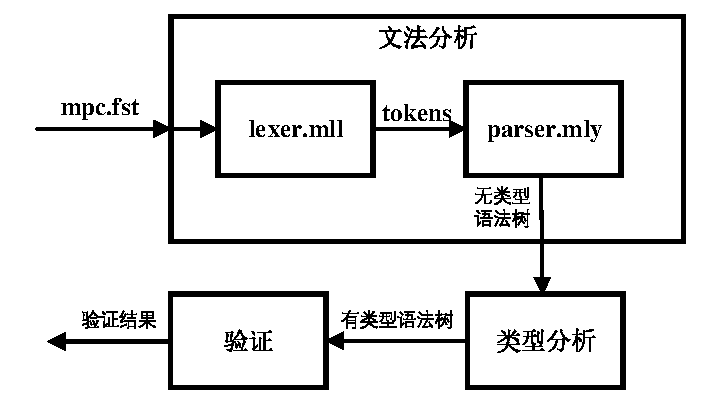
\includegraphics[width=0.70\textwidth]{sequence.pdf}
    \caption{Wys-ckt程序结构}
    \label{fig:sequence}
\end{figure}

Wys-ckt作为一环插入在整个程序验证部署环节当中,它接受一个经过Fstar验证的Wys*程序,验证完成后再经Fstar将程序编译为Ocaml或Fsharp目标代码,然后经由对应平台编译运行,Wys-ckt在整个验证部署环节中所处的位置如图\ref{fig:position_sequence}。

\begin{figure}[!htbp]
    \centering
    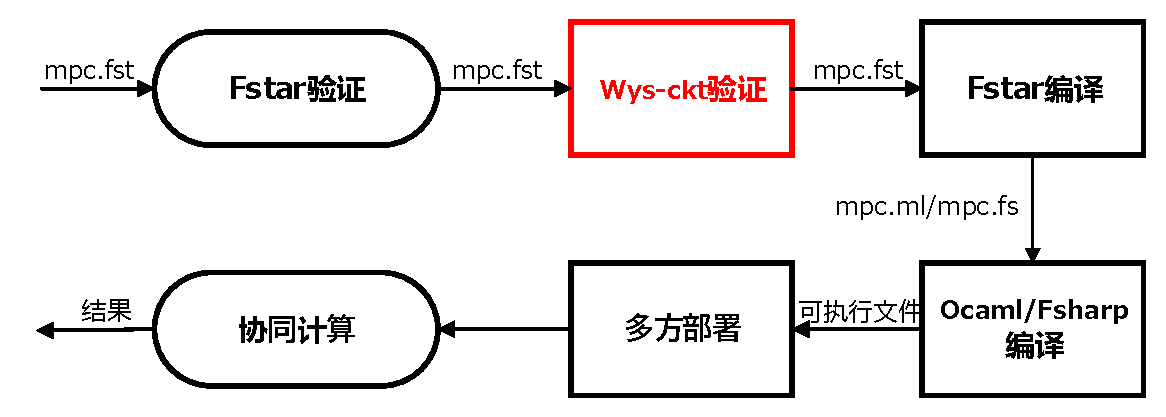
\includegraphics[width=1.00\textwidth]{sequence_all.pdf}
    \caption{Wys-ckt在Wys*程序验证部署流程中所处的位置}
    \label{fig:position_sequence}
\end{figure}

整个Wys-ckt的程序实现包含了大约500行Ocaml有效代码的文法分析部分,800行有效代码的语法树与类型分析部分,300行有效代码的验证部分,Wys-ckt的实际程序实现可以访问我的个人仓库https://github.com/YuXinFan/Wys-ckt获取。
\section{主要数据结构}
本文主要的数据结构包括两种语法树以及用于类型推导的记录结构化数据value和类型分析环境env。在一个纯函数式的程序当中的所有数值、变量、函数等元素都被看作与特定值绑定的命名量,因此声明一个如图\ref{fig:dvalue}结构式记录数据value记录每个命名量所绑定的值类型与所属的上下文环境。value中包含丰富的信息,每一个通过声明产生的变量都有一个value记录下它的名,所属类型,所属的环境,所包含的语法树。当通过声明产生一个函数时,value会额外记录函数的参数类型,返回类型,以及函数定义。value被用作有类型语法树重要基础组成,使有类型语法树包含了更丰富的信息。 
\begin{figure}[!htbp]
    \centering
    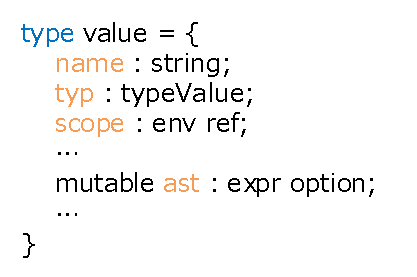
\includegraphics[width=0.50\textwidth]{dvalue.pdf}
    \caption{value结构记录的部分内容}
    \label{fig:dvalue}
\end{figure}
另一个结构式数据env如图\ref{fig:env}被用作类型分析时的环境,env中记录当前域的标识符和包含的所有类型作用域,一个env数据中不仅包含了当前环境的value数据、子作用域的env数据还记录了不同作用域之间的相对关系。当类型分析需要查询已有的命名变量的类型时,可以以名为关键字在当前环境和外部环境的env中查询获得所需要的信息。Wys-ckt通过创建一个拥有Env类型的只包含一个类型环境env字段的value数据,达到区别不同环境和变量在整个程序中所属的相对位置的目的。
\begin{figure}[!htbp]
    \centering
    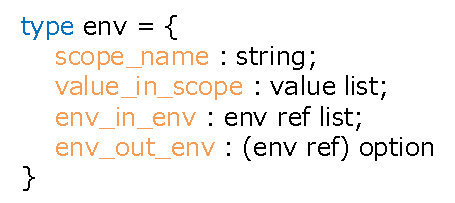
\includegraphics[width=0.50\textwidth]{env.pdf}
    \caption{env记录结构包含的字段}
    \label{fig:env}
\end{figure}
\section{语法树}
本部分分为三个阶段,第一阶段基于文法分析产生一个包含尽量多信息的预分析无类型语法树;第二阶段基于无类型语法树与类型推导规则进行类型推导;第三阶段重构一个结构更为清晰的有类型语法树。
\subsection{无类型语法树}
无类型语法树的构成有四层,程序层、声明层、表达式与类型声明层、命名变量层,每一层都按照文法规则设计,与3.1节中的语法一一对应。一个\textbf{module}语法与一系列decl声明语法共同组成一个完整的程序层。声明层包含四种声明分别对应\textbf{open}、\textbf{val}、\textbf{type}和\textbf{let}声明。表达式与类型声明层包含所有表达式种类以及函数定义时的参变量类型标识。命名变量层则用于记录变量、常数、匿名函数。

无类型语法树在文法分析过程中进行构建。分析一个Wys*的文法时会自动构建出一个分析树,这个分析树的结构与语法树对应。让文法分析树在每一个节点结束时生成一个对应结构的语法树节点,文法分析完成的同时一个无类型语法树也构建完成。
\subsection{静态类型分析}
无类型语法树中包含了一部分粗粒度处理过的信息(层级,表达式种类等)以及大部分的原始信息,这些信息需要加工后才能用于后续的分析工作,因此该部分的作用在于将其中的信息(尤其是类型信息)进行细化处理分类并进行按照类型推导规则填补空缺。

4.2节中数据结构主要就是为了解决这一部分问题,此部分的实现方法基于3.2节中的类型推导规则完成。所有的类型构建为一个联合结构,使用不同的类型名加以区分,然后遍历无类型语法树的每一个节点,按照3.2节的类型推导规则进行分析推导。对于一个叶节点上的值,首先匹配其模式是否为常数类型模式,如果是常数类型则按照所对应的模式分配类型,否则认为是一个命名变量类型。一个新的命名变量$v$由\textbf{let}声明或\textbf{let} \textbf{in}表达式产生,分析出它的类型等信息后将其名、类型、作用域、结构等信息组合成一个4.2中的value数据,并存入当前类型分析环境env中。当类型分析需要时,以名为关键字在当前环境中向上搜索即可得到包含$v$的所有信息在内的value数据。

在类型分析的过程中,对表达式层的分析占大部分内容。算法\ref{alg:exprtype}介绍本文实现的表达式层进行类型分析的方法。在算法\ref{alg:exprtype}中,\Call{TypeExpr}{}接受一个无类型语法树$ast$和类型环境$env$,返回$ast$的类型结果。\Call{TypeExpr}{}先从$ast$中获取根节点代表的表达式类型和各个子表达式,然后调用3.2节中描述的类型规则的具体实现函数\Call{TypeRule}{}完成类型推导。如3.2节中所描述的,\Call{TypeRule}{}包含每一种表达式的类型推导方法,由于篇幅原因本文算法\ref{alg:typerule}只展示\Call{TypeRule}{}的一部分内容。
\begin{algorithm}[!htbp]
    \small
    \caption{Expression Type Analysis Algorithm}\label{alg:exprtype}
    \hspace*{0.02in} {\bf Input:} \\
	\hspace*{0.04in} $ast$: The type-free abstract tree of the content of program \\
	\hspace*{0.04in} $env$: The typing environment containing types, methods, scopes \\
	\hspace*{0.02in} {\bf Output:} \\
	\hspace*{0.04in} The result type of the input expression
    \begin{algorithmic}[1]
        \Procedure{TypeExpr}{$env,ast$}
        \State $p\gets \text{pattern of } ast$ \Comment{获取输入表达式语法树$ast$的类型$p$}
        \State $m\gets \text{children of } ast$ \Comment{获得输入表达式语法树$ast$的所有次一级子树$m$}
        \State \Return \Call{TypeRule}{$env$,$p$,$m$} \Comment{调用类型推导规则的实现函数获得类型}
        \EndProcedure
    \end{algorithmic}
\end{algorithm}
\begin{algorithm}[!htbp]
    \small
    \caption{Partial of Type Rule Algorithm}\label{alg:typerule}
     \hspace*{0.02in} {\bf Input:} \\
	\hspace*{0.04in} $env$: The typing environment containing types, methods, scopes \\
	\hspace*{0.04in} $p$: The pattern expression type of an expression \\
	\hspace*{0.04in} $m$: A tuple containing abstract tree of sub-expressions \\
	\hspace*{0.02in} {\bf Output:} \\
	\hspace*{0.04in} The result type inferred from inputs
    \begin{algorithmic}[1]
        \Procedure{TypeRule}{$env,p,m$}
        \If {$p$=Constant}
        \State $c\gets \text{first of } m$ \Comment{从元组$m$中取得元素,常数节点$c$}
        \State \Return \Call{TypeConstant}{$c$} \Comment{匹配常数类型}
        \ElsIf {$p$=Variable}
        \State $x\gets \text{first of } m$ \Comment{从元组$m$中取得元素,变量节点$x$}
        \State \Return \Call{Find}{$env$,$x$}$.type$ \Comment{从env中查找$x$,并获得$x$的类型}
        \ElsIf {$p=$LetIn}
        \State $(x,e_1,e_2)\gets m$
        \State $env_2\gets env.sub\_env()$ \Comment{创建一个子环境}
        \State $env_2.value[x]\gets$ \Call{TypeExpr}{$env$, $e_1$}\Comment{在子环境中增加$x$对应的类型}
        \State \Return \Call{TypeExpr}{$env_2$, $e_2$} \Comment{LetIn表达式的类型取决于$e_2$}
        \ElsIf {$p=$IfCondition}
        \State $(b,e_1,e_2)\gets m$
        \State $typ \gets $\Call{TypeExpr}{$b$}
        \State $env_1\gets env.sub\_env()$ \Comment{创建子环境}
        \State $typ_1\gets$ \Call{TypeExpr}{$env_1$,$e_1$}\Comment{在子环境进行$e_1$的类型分析}
        \State $env_2\gets env.sub\_env()$
        \State $typ_2\gets$ \Call{TypeExpr}{$env_2$,$e_2$}
        \State \Return $typ_1$
        \ElsIf {...}
        \State {...}
        \EndIf 
        \EndProcedure
    \end{algorithmic}
\end{algorithm}
\subsection{有类型语法树}
有类型的语法树与无类型语法树的不同在于基础节点由原始字符信息变更为信息更为完整的value数据并且枝剪了不必要的细化类型信息。有类型语法树的结构框架仍依照无类型语法树,静态分析时产生的各个value数据不断填补到语法树的对应位置即能完成有类型语法树的构建。
\section{验证函数}
获得完整的有类型信息的语法树之后,得益于ML家族的模式匹配特性,验证函数的实现过程十分方便。\Call{CheckingRule}{}实现了3.3节中描述的不同表达式所受到的类型限制的检查,\Call{CheckingRule}{}也使用模式匹配和分支的结构,与算法\ref{alg:typerule}的形式类似。算法\ref{alg:verify}描述了对安全计算函数进行验证的方法。在完整的验证过程中,Wys-ckt通过遍历搜索定位程序中的\textbf{as\_sec} $ps$ $g$语句,$g$即为待验证的安全计算函数的名,然后以$g$为关键字在语句所在的上下文环境中找出$g$所定义的表达式内容,该表达式对应的语法树$ast$即为待验证的安全计算函数表达式的等价语法树,$ast$将作为函数输入参数传递给验证函数verify\_as\_sec。verify\_as\_sec调用算法\ref{alg:verify}和\Call{CheckingRule}{}的实际实现函数verify\_ast\_expr完成对安全计算函数的验证。
\begin{algorithm}[!htbp]
    \small
    \caption{Verification Algorithm}\label{alg:verify}
    \hspace*{0.02in} {\bf Input:} \\
	\hspace*{0.04in} $ast$: the typed abstract tree of the content of secure function \\
	\hspace*{0.02in} {\bf Output:} \\
	\hspace*{0.04in} $true$ means succeed,vice versa.
    \begin{algorithmic}[1]
        \Procedure{VerifyExpr}{$ast$}
        \State $p\gets \text{pattern of } ast$ \Comment{获取表达式语法树$ast$的类型$p$}
        \State $m\gets \text{children of } ast$ \Comment{获取表达式语法树$ast$的所有次一级子树$m$}
        \State $r\gets$ \Call{CheckingRule}{$p$,$m$} \Comment{调用验证规则算法检查$m$和$p$是否符合验证规则}
        \For{each subtree $i$ in $m$}
        \State $s\gets$ \Call{VerifyExpr}{$i$} \Comment{依次验证每一个子表达式}
        \If {$s=false$}
        \State \Return $false$
        \EndIf
        \EndFor
        \State \Return $r$
        \EndProcedure
    \end{algorithmic}
\end{algorithm}
\chapter{总结与展望}
多方安全计算协议经过不断研究诞生了如GMW协议、BMR协议、PSSZ协议等一系列具有较高效率的实用协议,由于多方安全计算的实际需求也出现了Sharemind、Obliv-C、ABY等接近十种程序开发框架。形式化的验证多方计算程序和框架对提高安全性有重要的意义。本文基于对多方安全计算领域特定语言Wys*的分析,观察Wys*在形式化验证自身时遗留下的问题,设计和实现了一种基于类型系统的在Wys*进行电路翻译前验证待翻译的程序语义是否符合Wys*翻译能力的方法,作为Wys*验证链的补充。其他验证工作如SecreC也有相似的问题,因此本文的方法也为解决这一类问题提供了思路。根据文献调查,目前对多方安全计算程序进行形式化验证的工作只有有限的几篇文献\citep{almeida2018enforcing,rastogi2019textsc,rastogi2017wys}。多方安全计算程序区别与一般的逻辑程序,涉及网络、电路、安全协议等方方面面,对多方安全计算程序和框架进行完整的形式化验证仍有极大的研究空间。
基于本文设计的验证方法和研究过程中对多方安全计算程序验证工作的分析,后续的研究工作可以从以下方向进行:
\begin{itemize}
\item 设计具有完整的隐私数据信息流安全性验证和程序正确性验证的多方安全计算程序验证方案,目前研究领域的验证工作中只关注隐私数据的安全性或者程序正确性而没有进行结合,丧失了整体的可靠性。
\item 对一个布尔电路翻译模块进行形式化验证,以Wys*所使用的翻译算法为例\citep{choi2012secure},先验证该翻译算法的正确性,然后基于该算法的某一主要实现验证该实现的正确性。
\item 验证一个多方安全计算协议程序实现的正确性,这是一个具有挑战性的研究方向,目前研究领域还没有与该方向直接相关的成果。
\item 证明Wys*的底层语义的安全性,这一部分内容较多的涉及Wys*所依赖的Fstar,需要证明Wys*与Fstar的核心语义具有完整的对应关系。
\end{itemize}


%---------------------------------------------------------------------------%
% main content
	%-
	%-> Appendix
	%-
	\cleardoublepage%
	\appendix% initialize the environment
	%\chapter{中国科学院大学学位论文撰写要求}

学位论文是研究生科研工作成果的集中体现,是评判学位申请者学术水平、授予其学位的主要依据,是科研领域重要的文献资料。根据《科学技术报告、学位论文和学术论文的编写格式》(GB/T 7713-1987)、《学位论文编写规则》(GB/T 7713.1-2006)和《文后参考文献著录规则》(GB7714—87)等国家有关标准,结合中国科学院大学(以下简称“国科大”)的实际情况,特制订本规定。

\section{论文无附录者无需附录部分}

\section{测试公式编号} \label{sec:testmath}

\begin{equation} \label{eq:appedns}
    \begin{cases}
        \frac{\partial \rho}{\partial t} + \nabla\cdot(\rho\Vector{V}) = 0 \ \mathrm{times\ font\ test}\\
        \frac{\partial (\rho\Vector{V})}{\partial t} + \nabla\cdot(\rho\Vector{V}\Vector{V}) = \nabla\cdot\Tensor{\sigma} \ \text{times font test}\\
        \frac{\partial (\rho E)}{\partial t} + \nabla\cdot(\rho E\Vector{V}) = \nabla\cdot(k\nabla T) + \nabla\cdot(\Tensor{\sigma}\cdot\Vector{V})
    \end{cases}
\end{equation}
\begin{equation}
    \frac{\partial }{\partial t}\int\limits_{\Omega} u \, \mathrm{d}\Omega + \int\limits_{S} \unitVector{n}\cdot(u\Vector{V}) \, \mathrm{d}S = \dot{\phi}
\end{equation}

\section{测试生僻字}

霜蟾盥薇曜灵霜颸妙鬘虚霩淩澌菀枯菡萏泬寥窅冥毰毸濩落霅霅便嬛岧峣瀺灂姽婳愔嫕飒纚棽俪緸冤莩甲摛藻卮言倥侗椒觞期颐夜阑彬蔚倥偬澄廓簪缨陟遐迤逦缥缃鹣鲽憯懔闺闼璀错媕婀噌吰澒洞阛闠覼缕玓瓑逡巡諓諓琭琭瀌瀌踽踽叆叇氤氲瓠犀流眄蹀躞赟嬛茕頔璎珞螓首蘅皋惏悷缱绻昶皴皱颟顸愀然菡萏卑陬纯懿犇麤掱暒 墌墍墎墏墐墒墒墓墔墕墖墘墖墚墛坠墝增墠墡墢墣墤墥墦墧墨墩墪樽墬墭堕墯墰墱墲坟墴墵垯墷墸墹墺墙墼墽垦墿壀壁壂壃壄壅壆坛壈壉壊垱壌壍埙壏壐壑壒压壔壕壖壗垒圹垆壛壜壝垄壠壡坜壣壤壥壦壧壨坝塆圭嫶嫷嫸嫹嫺娴嫼嫽嫾婳妫嬁嬂嬃嬄嬅嬆嬇娆嬉嬊娇嬍嬎嬏嬐嬑嬒嬓嬔嬕嬖嬗嬘嫱嬚嬛嬜嬞嬟嬠嫒嬢嬣嬥嬦嬧嬨嬩嫔嬫嬬奶嬬嬮嬯婴嬱嬲嬳嬴嬵嬶嬷婶嬹嬺嬻嬼嬽嬾嬿孀孁孂娘孄孅孆孇孆孈孉孊娈孋孊孍孎孏嫫婿媚嵭嵮嵯嵰嵱嵲嵳嵴嵵嵶嵷嵸嵹嵺嵻嵼嵽嵾嵿嶀嵝嶂嶃崭嶅嶆岖嶈嶉嶊嶋嶌嶍嶎嶏嶐嶑嶒嶓嵚嶕嶖嶘嶙嶚嶛嶜嶝嶞嶟峤嶡峣嶣嶤嶥嶦峄峃嶩嶪嶫嶬嶭崄嶯嶰嶱嶲嶳岙嶵嶶嶷嵘嶹岭嶻屿岳帋巀巁巂巃巄巅巆巇巈巉巊岿巌巍巎巏巐巑峦巓巅巕岩巗巘巙巚帠帡帢帣帤帨帩帪帬帯帰帱帲帴帵帷帹帺帻帼帽帾帿幁幂帏幄幅幆幇幈幉幊幋幌幍幎幏幐幑幒幓幖幙幚幛幜幝幞帜幠幡幢幤幥幦幧幨幩幪幭幮幯幰幱庍庎庑庖庘庛庝庠庡庢庣庤庥庨庩庪庬庮庯庰庱庲庳庴庵庹庺庻庼庽庿廀厕廃厩廅廆廇廋廌廍庼廏廐廑廒廔廕廖廗廘廙廛廜廞庑廤廥廦廧廨廭廮廯廰痈廲廵廸廹廻廼廽廿弁弅弆弇弉弖弙弚弜弝弞弡弢弣弤弨弩弪弫弬弭弮弰弲弪弴弶弸弻弼弽弿彖彗彘彚彛彜彝彞彟彴彵彶彷彸役彺彻彽彾佛徂徃徆徇徉后徍徎徏径徒従徔徕徖徙徚徛徜徝从徟徕御徢徣徤徥徦徧徨复循徫旁徭微徯徰徱徲徳徴徵徶德徸彻徺忁忂惔愔忇忈忉忔忕忖忚忛応忝忞忟忪挣挦挧挨挩挪挫挬挭挮挰掇授掉掊掋掍掎掐掑排掓掔掕挜掚挂掜掝掞掟掠采探掣掤掦措掫掬掭掮掯掰掱掲掳掴掵掶掸掹掺掻掼掽掾掿拣揁揂揃揅揄揆揇揈揉揊揋揌揍揎揑揓揔揕揖揗揘揙揤揥揦揧揨揫捂揰揱揲揳援揵揶揷揸揻揼揾揿搀搁搂搃搄搅搇搈搉搊搋搌搎搏搐搑搒摓摔摕摖摗摙摚摛掼摝摞摠摡斫斩斮斱斲斳斴斵斶斸旪旫旮旯晒晓晔晕晖晗晘晙晛晜晞晟晠晡晰晣晤晥晦晧晪晫晬晭晰晱晲晳晴晵晷晸晹晻晼晽晾晿暀暁暂暃暄暅暆暇晕晖暊暋暌暍暎暏暐暑暒暓暔暕暖暗旸暙暚暛暜暝暞暟暠暡暣暤暥暦暧暨暩暪暬暭暮暯暰昵暲暳暴暵暶暷暸暹暺暻暼暽暾暿曀曁曂曃晔曅曈曊曋曌曍曎曏曐曑曒曓曔曕曗曘曙曚曛曜曝曞曟旷曡曢曣曤曥曦曧昽曩曪曫晒曭曮曯椗椘椙椚椛検椝椞椟椠椡椢椣椤椥椦椧椨椩椪椫椬椭椮椯椰椱椲椳椴椵椶椷椸椹椺椻椼椽椾椿楀楁楂楃楅楆楇楈楉杨楋楌楍榴榵榶榷榸榹榺榻榼榽榾桤槀槁槂盘槄槅槆槇槈槉槊构槌枪槎槏槐槑槒杠槔槕槖槗滙滛滜滝滞滟滠滢滣滦滧滪滫沪滭滮滰滱渗滳滵滶滹滺浐滼滽漀漃漄漅漈漉溇漋漌漍漎漐漑澙熹漗漘漙沤漛漜漝漞漟漡漤漥漦漧漨漪渍漭漮漯漰漱漳漴溆漶漷漹漺漻漼漽漾浆潀颍潂潃潄潅潆潇潈潉潊潋潌潍潎潏潐潒潓洁潕潖潗潘沩潚潜潝潞潟潠潡潢潣润潥潦潧潨潩潪潫潬潭浔溃潱潲潳潴潵潶滗潸潹潺潻潼潽潾涠澁澄澃澅浇涝澈澉澊澋澌澍澎澏湃澐澑澒澓澔澕澖涧澘澙澚澛澜澝澞澟渑澢澣泽浍澯澰淀澲澳澴澵澶澷澸潇潆瀡瀢瀣瀤瀥潴泷濑瀩瀪瀫瀬瀭瀮瀯弥瀱潋瀳瀴瀵瀶瀷瀸瀹瀺瀻瀼瀽澜瀿灀灁瀺灂沣滠灅灆灇灈灉灊灋灌灍灎灏灐洒灒灓漓灖灗滩灙灚灛灜灏灞灟灠灡灢湾滦灥灦灧灨灪燝燞燠燡燢燣燤燥灿燧燨燩燪燫燮燯燰燱燲燳烩燵燵燸燹燺薰燽焘燿爀爁爂爃爄爅爇爈爉爊爋爌烁爎爏爑爒爓爔爕爖爗爘爙爚烂爜爝爞爟爠爡爢爣爤爥爦爧爨爩猽猾獀犸獂獆獇獈獉獊獋獌獍獏獐獑獒獓獔獕獖獗獘獙獚獛獜獝獞獟獠獡獢獣獤獥獦獧獩狯猃獬獭狝獯狞獱獳獴獶獹獽獾獿猡玁玂玃。
% appendix content
	%-
	%-> Backmatter: bibliography, glossary, index
	%-
	\backmatter% initialize the environment
	\intotoc{\bibname}% add link to contents table and bookmark
	\bibliography{Biblio/ref}% bibliography
	%\chapter{作者简历及攻读学位期间发表的学术论文与研究成果}
%
%\textbf{本科生无需此部分}。
%
%\section*{作者简历}
%
%\subsection*{casthesis作者}
%
%吴凌云,福建省屏南县人,中国科学院数学与系统科学研究院博士研究生。
%
%\subsection*{ucasthesis作者}
%
%莫晃锐,湖南省湘潭县人,中国科学院力学研究所硕士研究生。
%
%\section*{已发表(或正式接受)的学术论文:}
%
%[1] ucasthesis: A LaTeX Thesis Template for the University of Chinese Academy of Sciences, 2014.
%
%\section*{申请或已获得的专利:}
%
%(无专利时此项不必列出)
%
%\section*{参加的研究项目及获奖情况:}
%
%可以随意添加新的条目或是结构。

\chapter[致谢]{致\quad 谢}\chaptermark{致\quad 谢}% syntax: \chapter[目录]{标题}\chaptermark{页眉}
%\thispagestyle{noheaderstyle}% 如果需要移除当前页的页眉
%\pagestyle{noheaderstyle}% 如果需要移除整章的页眉
%\pagestyle{mainmatterstyle} % 与前文页眉页脚格式相同
本论文是在我的导师宋富教授的悉心指导之下完成的。本论文在选题、调研和确定具体内容等诸多方面都受到了宋老师的悉心帮助。本科时学习的宋老师授课的编译原理课程对本文设计研究方法和推进程序实现起到了重要的作用。宋老师踏实严谨的治学态度引导我步入学术研究生涯,令我终生受益。在此我对宋老师表示由衷的感谢!

我要感谢我的家人!感谢父母对我的支持,在生活和学习上都给予了无微不至的帮助,让我在疫情期间依然能将精神集中于本论文的设计撰写。

感谢我的学长学姐、同门的师兄弟以及各位教授,有你们的帮助和教育我才有能力不断的解决困难。我们在上科大度过的学习生活时光会成为我生命中宝贵的记忆。感谢我的同学与我分享快乐,也陪我经历磨难。感谢我的室友一直以来的照顾。

最后我要感谢母校上海科技大学!立志,成才,报国,裕民八字校训每次思考都让我有不同的体悟。感谢信息学院的老师们在学习、生活上提供的指导。感谢四年来我在上科大求学生涯的每一位参与者!

\cleardoublepage[plain]% 让文档总是结束于偶数页,可根据需要设定页眉页脚样式,如 [noheaderstyle]

% other information
\end{document}
%---------------------------------------------------------------------------%

